%!TEX encoding = UTF-8 Unicode
%!TEX root = ../lect-w10.tex

%%%


%\begin{Slide}{TODO: Begrepp att förklara}
%  Tänk igenom ordningen:
%  \begin{itemize}
%    \item java switch, scala match ... 
%  \end{itemize}
%\end{Slide}
%
%
%\begin{Slide}{Javas switch-sats}
%A switch in Java works with the byte, short, char, and int primitive data types. It also works with enumerated types (discussed in Enum Types), the String class, and a few special classes that wrap certain primitive types: Character, Byte, Short, and Integer
%\end{Slide}


\Subsection{Veckans lab: \texttt{chords-team}}
\begin{Slide}{Veckans lab: \texttt{chords-team}}\SlideFontSmall
Övergripande syfte:
\begin{itemize}
\item Träna på case-klasser, matchning, undantag
\item Jobba med ett större program med flera delar i olika filer
\item Jobba flera personer på samma program
\end{itemize}
Innehåll:
\begin{itemize}
\item Skapa och spara ackord på gitarr (6 strängar) och ukulele (4 strängar) 
\item Spela upp ackord med Javas inbyggda musikspelare inkapslad i \code{SimpleNotePlayer}
\item Rita ackord med \code{SimpleWindow} 
\end{itemize}
Hur mycket ni gör beror på hur många ni är i gruppen och hur stora ambitioner ni har. Diskutera detta med handledare på resurstid.
\end{Slide}

\begin{Slide}{Toner, oktaver och ackord}\SlideFontSmall
\begin{itemize}
\item Det finns 12 toner som har speciella namn: \\ C, C\#, D, D\#, etc. (uttalas: c, ciss, d, diss, etc.)
\item Jämför vita och svarta tangenter på ett piano: \\ avståndet mellan varje tangent är ett s.k. \emph{halvt tonsteg}. 
\item Toner återkommer i oktaver, modulo 12.
\item Tonen som representeras av strängen \code{"D2"} är tonen D i andra oktaven.
\item Tonen \code{"D2"} motsvarar heltalet \code{26} på labben.
\item Ett ackord består av flera toner.
\end{itemize}
\begin{REPL}[basicstyle=\color{white}\ttfamily\SlideFontSize{6}{7}\selectfont]
scala> val notes = Vector("C", "C#", "D", "D#", "E", "F", "F#", "G", "G#", "A", "A#", "B")

scala> notes.size
res0: Int = 12

scala> notes(26 % 12)
res1: String = D

\end{REPL}
\end{Slide}

\begin{Slide}{Toner på ett stränginstrument}
\begin{minipage}{0.5\textwidth}
\begin{itemize}\SlideFontSmall
\item Gitarr och ukulele har 6 resp. 4 strängar och en greppbräda med s.k. band.

\item Om man trycker ned ett finger på (egentligen bakom) första bandet höjs tonen ett halvt tonsteg. 

\item Exempel: om en sträng är stämd i D3 blir tonen om man trycker ned fingret på fjärde bandet F\#3.

\item \href{http://www.gitarr.org}{www.gitarr.org}

\item \href{http://www.stefansukulele.com}{www.stefansukulele.com}

\end{itemize}
\end{minipage}
\begin{minipage}{0.45\textwidth}
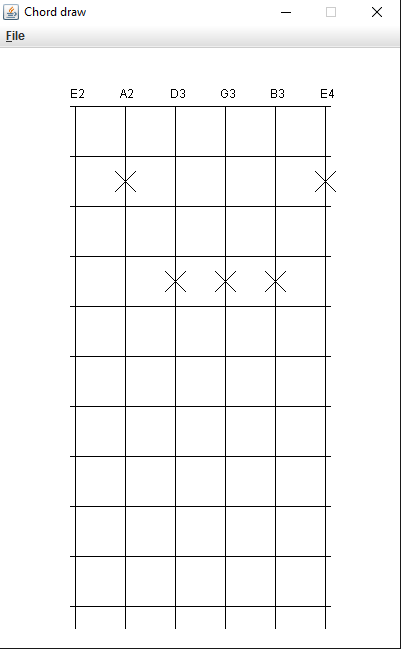
\includegraphics[width=1.0\textwidth]{../img/chords/ChordDraw}
\end{minipage}

\end{Slide}

\begin{Slide}{Modell av gitarr och ukulele}
\begin{Code}
object model {

  type Tuning = Vector[String]
  type Grip = Vector[Int]

  trait Chord {
    def name: String
    def tuning: Tuning
    def grip: Grip
  }
  
  case class Guitar(name: String, grip: Grip) extends Chord {
    val tuning = Vector("E2", "A2", "D3", "G3", "B3", "E4")
  }
  
  case class Ukulele(name: String, grip: Grip) extends Chord {
    val tuning = Vector("G4", "C4", "E4", "A4")
  }

}
\end{Code}
\end{Slide}

\begin{Slide}{En gemensam bastyp för olika ackord}\SlideFontSmall
\vspace{-0.5em}\begin{center}
\newcommand{\TextBox}[1]{\raisebox{0pt}[1em][0.5em]{#1}}
\tikzstyle{umlclass}=[rectangle, draw=black,  thick, anchor=north, text width=3cm, rectangle split, rectangle split parts = 3]
\begin{tikzpicture}[inner sep=0.5em]
\node [umlclass, rectangle split parts = 2, xshift=0cm, text width=5cm] (BaseType)  {
            \textit{\textbf{\centerline{\TextBox{\code{Chord}}}}}
            \nodepart[]{second}
            \TextBox{\code{def name: String}}\vspace{-0.25em}\newline
            \TextBox{\code{def tuning: Vector[String]}}\vspace{-0.25em}\newline
            \TextBox{\code{def grip: Vector[Int]}}\vspace{-0.25em}\newline

        };
        
\node [umlclass, rectangle split parts = 1]  at (2.5cm,-3.7cm) (SubType1) {
            \textbf{\centerline{\TextBox{\code{Guitar}}}}
            %\nodepart[]{second} \TextBox{~}
        };  
                
\node [umlclass, rectangle split parts = 1] at (-2.5cm,-3.7cm) (SubType2)  {
            \textbf{\centerline{\TextBox{\code{Ukulele}}}}
            %\nodepart[]{second} \TextBox{talk(): void}
        };        
\draw[umlarrow] (SubType1.north) -- ++(0,0.5) -| (BaseType.south);    
\draw[umlarrow] (SubType2.north) -- ++(0,0.5) -| (BaseType.south);            
\end{tikzpicture}
\end{center}
\pause\vspace{-0.7em}
\begin{REPL}
scala> import model._

scala> val uc = Ukulele("C", Vector(0, 0, 0, 3))
uc: model.Ukulele = Ukulele(C,Vector(0, 0, 0, 3))

scala> val ge = Guitar("E", Vector(0, 2, 2, 1, 0, 0))
ge: model.Guitar = Guitar(E,Vector(0, 2, 2, 1, 0, 0))
\end{REPL}
\end{Slide}


\begin{Slide}{Grupparbete}\SlideFontSmall
\begin{itemize}
\item Förslag på arbetssätt:
\begin{itemize}\SlideFontSmall
\item Träffas nu på rasten och boka nästa gruppmöte
\item Förberedelser inför första gruppmötet: individuella studier av labbinstruktioner och koden som är given i workspace \\
\href{https://github.com/lunduniversity/introprog/tree/master/workspace/w08_chords_team/src}{.../workspace/w08\_chords\_team/src} \\
OBS! numrering av labbarna enl. ''gamla'' veckor
\item Träffas gärna i ett studierum med whiteboard
\item På mötet: gå igenom uppgift och given kod så att alla fattar vad det går ut på; bestäm omfattning och ansvarsuppdelning
\item När ni träffas, skissa upp den kod som just du håller på med på whiteboard och få feedback och ge feedback till andra
\item På varje gruppmöte, bestäm tid för nästa möte och vad var och en ska försöka hinna tills dess
\end{itemize}


\item Ni får \Emph{lov att ändra på omfattningen} efter antalet gruppmedlemmar, ambition och förmåga: diskutera detta med handledare på resurstid

\item \Alert{Minimikrav}: att med textkommando kunna skapa/spara/ladda gitarr- och ukulele-ackord och att ni tränar på matchning

\end{itemize}
\end{Slide}


\Subsection{Matchning}

\begin{Slide}{Vad är matchning?}
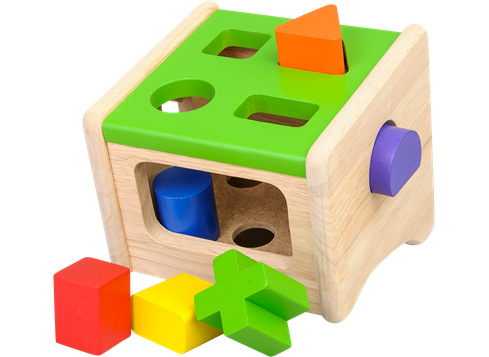
\includegraphics[width=0.8\textwidth]{../img/plocklada.png}
\end{Slide}


\begin{Slide}{Vad är matchning?}
Matchning gör man då man vill jämföra ett värde mot andra värden och hitta överensstämmelse \Eng{match}.

\pause

\vspace{1em}Detta kan man t.ex. göra med nästlade if-else-satser/uttryck:

\begin{Code}
val g = scala.io.StdIn.readLine("grönsak:")
val smak = 
  if (g == "gurka") "gott!"
  else if (g == "tomat") "jättegott!"
  else if (g == "broccoli") "ganska gott..."
  else "inte gott :("

println(g + " är " + smak)
\end{Code}
\end{Slide}




\begin{Slide}{Javas switch-sats}\SlideFontSmall
De flesta C-liknande språk (men inte Scala) har en \jcode{switch}-sats som man kan använda istället för (vissa) nästlade if-else-satser: 
\javainputlisting[basicstyle=\ttfamily\SlideFontSize{5.5}{6.8}\selectfont]{../compendium/examples/match/Switch.java}

\vspace{-0.5em}Funkar bara för primitiva typer och några till (t.ex. String).
\end{Slide}




\begin{Slide}{Javas switch-sats utan break}\SlideFontSmall
Saknad \jcode{break}-sats ''faller igenom'' till efterföljande gren: 

\javainputlisting[basicstyle=\ttfamily\SlideFontSize{6}{7}\selectfont]{../compendium/examples/match/SwitchNoBreak.java}
En glömd \jcode{break} kan ge svårhittad bugg... 
\end{Slide}

\begin{Slide}{Javas switch-sats med glömd break}\SlideFontSmall

\vspace{-0.5em}\javainputlisting[basicstyle=\ttfamily\SlideFontSize{5.5}{6.8}\selectfont]{../compendium/examples/match/SwitchForgotBreak.java}

\vspace{-0.7em}\pause
\begin{REPL}
$ java SwitchForgotBreak 
Skriv grönsak:
gurka
gott!
gott!
\end{REPL}

\end{Slide}


\begin{Slide}{Scalas \texttt{match}-uttryck}\SlideFontSmall
Scala har ingen \code{switch}-sats men erbjuder i stället ett \code{match}-\Emph{uttryck} som är kraftfullare och ger ett värde.

\begin{Code}
val g = scala.io.StdIn.readLine("grönsak:")
val smak = g match {
  case "gurka" => "gott!"
  case "tomat" => "jättegott!"
  case "broccoli" => "ganska gott..."
  case _ => "mindre gott..."
}
println(g + " är " + smak)
\end{Code}
Och den ''faller inte igenom'' som Javas \code{switch}-sats! 
\begin{itemize}
\pause\item Varje \code{case}-gren testas var för sig i tur och ordning uppifrån och ned.
\pause\item Det som står mellan \code{case} och \code{=>} kallas ett \Emph{mönster} \Eng{pattern}
\pause\item Sista default-grenen ovan kallas \Emph{wildcard-mönster}: \code{case _ => } 
\pause\item Ovan är exempel på matchning mot \Emph{konstant-mönster}, \\ i detta fallet tre stycken strängkonstantmönster.
\pause\item Det finns många andra sätt att skriva mönster.
\end{itemize}
\end{Slide}



\begin{Slide}{Matchning med gard}
Man kan stoppa in en s.k \Emph{gard} \Eng{guard} innan pilen \code{=>} för att villkora matchningen: (notera \code{if}, parenteser behövs ej)
\begin{Code}
val g = scala.io.StdIn.readLine("grönsak:")
def f = g match {
  case "gurka" if math.random > 0.5 => "gott ibland!"
  case "tomat" => "jättegott!"
  case "broccoli" => "ganska gott..."
  case _ => "mindre gott..."
}
\end{Code}
\code{case}-grenen med gard ger bara en lyckad matchning \\ om uttrycket efter \code{if} är sant; annars provas nästa gren, etc.
\end{Slide}

\begin{Slide}{Matchning med variabelmönster}\SlideFontSmall
Om det finns ett namn efter \code{case} som börjar med liten begynnelsebokstav, blir detta namn en variabel som automatiskt binds till uttrycket före \code{match}:

\begin{Code}
val g = scala.io.StdIn.readLine("grönsak:")
def f = g match {
  case "gurka" if math.random > 0.5 => "gott ibland!"
  case "tomat" => "jättegott!"
  case "broccoli" => "ganska gott..."
  case other => "smakar bakvänt: " + other.reverse
}
\end{Code}

Ett enkelt variabelmönster, så som \\ \code{case other => ...} \\ i exemplet ovan, matchar \Emph{allt}! \\\code{other} får alltså värdet av \code{g} om \code{g} \Alert{inte} är \code{"gurka"}, \code{"tomat"}, \code{"broccoli"}.  

\end{Slide}





\begin{Slide}{Matchning med typade mönster}\SlideFontSmall
Med en typannotering efter en variabel får man ett \Emph{typat mönster} \Eng{typed pattern}. Om matchningen lyckas blir värdet \Alert{omvandlat} till den specifika typen och binds till variabeln.
\begin{Code}
def f = if (math.random < 0.5) 42 + math.random else "gurka" + math.random
def g = f match {
  case x: Double => x.round.toInt
  case s: String => s.length
}
\end{Code}
Vad har funktionen \code{f} för returtyp? \\ \pause
Matchning mot specifika typer enl. ovan används i idiomatisk Scala hellre än \code{isInstanceOf} men man kan göra motsvarande ovan med if-uttryck:
\begin{Code}
def g2 = {
  val x = f
  if (x.isInstanceOf[Double]) x.asInstanceOf[Double].round.toInt
  else if (x.isInstanceOf[String]) x.asInstanceOf[String].length
}.asInstanceOf[Int]
\end{Code}
\end{Slide}


\begin{Slide}{Konstruktormönster med case-klasser}\SlideFontSmall
En basklass med gemensamma delar och två subtyper:
\begin{Code}
trait Grönsak {
  def vikt: Int
  def ärRutten: Boolean
}
case class Gurka(vikt: Int, ärRutten: Boolean) extends Grönsak
case class Tomat(vikt: Int, ärRutten: Boolean) extends Grönsak
\end{Code}
\pause
Tack vare case-klasserna kan man använda \Emph{konstruktormönster} \Eng{constructor pattern} för att kolla vad som finns \Alert{inuti} en instans:
\begin{Code}
def testa(g: Grönsak): String = g match {
  case Gurka(v, false) => "gott, väger " + v
  case Gurka(_, true)  => "inte gott"
  case Tomat(v, r)     => (if (r) "inte " else "") + "gott, väger " + v 
  case _ => "okänd grönsak: " + g
}
\end{Code}

Konstruktormönster ''\Emph{plockar isär}'' det som matchas och binder variabler till de attribut som finns i case-klassens konstruktor.
\end{Slide}


\begin{Slide}{Plocka isär samlingar med djupa mönster}
Man kan plocka isär innehållet i en samling så här:
\begin{Code}
def visa(xs: Vector[Grönsak]): String = xs match {
  case Vector()               => "tom grönsaksvektor"
  case Vector(Gurka(v, true)) => "en rutten gurka som väger " + v
  case Vector(g)              => "exakt en grönsak: " + g
  case Vector(g1, g2)         => s"exakt två grönsaker: $g1, $g2"
  case g +: gs                => s"först en $g och sedan svansen: $gs" 
}
\end{Code}
Övning: prova ovan i REPL. Vad händer om du byter ordning på andra och tredje mönstret ovan?
\end{Slide}

\begin{Slide}{Mönstermatchning och case-objekt}
En bastyp och specifika singelobjekt av gemensam typ:
\begin{Code}
trait Färg
case object Spader  extends Färg
case object Hjärter extends Färg
case object Ruter   extends Färg
case object Klöver  extends Färg

def parallellFärg(f: Färg): Färg = f match {
  case Spader  => Klöver
  case Klöver  => Spader
  case Hjärter => Ruter
}
\end{Code}
Vilken case-gren har vi glömt? Kan kompilatorn hjälpa oss?
\pause
\begin{REPL}
scala> parallellFärg(Ruter)
scala.MatchError: Ruter (of class Ruter$)
  at .parallellFärg(<console>:18)

\end{REPL}
Runtime exception \code{:(} ~~och en bugg som kan vara svårhittad...
\end{Slide}

\begin{Slide}{Mönstermatchning och förseglade typer}
Med nyckelordet \code{sealed} får vi en kompileringsvarning \code{:)}
\begin{Code}
sealed trait Färg
case object Spader  extends Färg
case object Hjärter extends Färg
case object Ruter   extends Färg
case object Klöver  extends Färg

def parallellFärg(f: Färg): Färg = f match {
  case Spader  => Klöver
  case Klöver  => Spader
  case Hjärter => Ruter
}
\end{Code}
\begin{REPL}
// Exiting paste mode, now interpreting.

<console>:23: warning: match may not be exhaustive.
It would fail on the following input: Ruter
       def parallellFärg(f: Färg): Färg = f match {
\end{REPL}
\end{Slide}

\begin{Slide}{Stora/små begynnelsebokstäver vid matchning}
Fallgrop: att försöka matcha på värdet av en variabel som börjar med liten bokstav.
\begin{REPL}
scala> val livetsMening = 42

scala> def ärLivetsMeningBuggig(svar: Int) = svar match {
         case livetsMening => true    // lokalt namn som matchar allt!
         case _ => false
       }

scala> ärLivetsMeningBuggig(43)
res0: Boolean = true

scala> val LivetsMening = 42   // stor begynnelsebokstav

scala> def ärLivetsMening(svar: Int) = svar match {
         case LivetsMening => true    // funkar fint!
         case _ => false
       }

scala> ärLivetsMening(43)
res1: Boolean = false
\end{REPL}
\end{Slide}


\begin{Slide}{Stora/små begynnelsebokstäver vid matchning}
Ett sätt att komma runt problemet med liten begynnelsebokstav: \\
\Emph{backticks} to the rescue!
\begin{REPL}
scala> val livetsMening = 42

scala> def ärLivetsMeningBackTicks(svar: Int) = svar match {
         case `livetsMening` => true    // nu funkar det!
         case _ => false
       }

scala> ärLivetsMeningBackTicks(43)
res2: Boolean = false
\end{REPL}
\end{Slide}


\begin{Slide}{Mönster på andra ställen än i \texttt{match}}\SlideFontSmall
Mönster i \Emph{deklarationer}:
\vspace{-0.25em}\begin{REPL}
scala> case class Point(x: Int, y: Int)

scala> val p = Point(0, 1)

scala> val Point(x, y) = p          // konstruktormönster med case-klass
x: ???
y: ???

scala> val (x, y, z) = (0, 1, 2)    // konstruktormönster med tupel
x: ???
y: ???
z: ???

\end{REPL}
Mönster i \Emph{for-satser}:
\vspace{-0.25em}\begin{REPL}
scala> val xs = for ((x, y) <- Vector((1,2), (3,4))) yield x
xs: ???
\end{REPL}

\end{Slide}

\begin{Slide}{Mönster på andra ställen än i \texttt{match}}\SlideFontSmall
Mönster i \Emph{deklarationer}:
\vspace{-0.25em}\begin{REPL}
scala> case class Point(x: Int, y: Int)

scala> val p = Point(0, 1)

scala> val Point(x, y) = p          // konstruktormönster med case-klass
x: Int = 0
y: Int = 1

scala> val (x, y, z) = (0, 1, 2)    // konstruktormönster med tupel
x: Int = 0
y: Int = 1
z: Int = 2

\end{REPL}
Mönster i \Emph{for-satser}:
\vspace{-0.25em}\begin{REPL}
scala> val xs = for ((x, y) <- Vector((1,2), (3,4))) yield x
xs: scala.collection.immutable.Vector[Int] = Vector(1, 3)
\end{REPL}
\end{Slide}

\begin{Slide}{Fördjupning om mönster}
Avancerade saker för den intresserade (ingår ej): 
\begin{itemize}
\item binda variabler till mönsterdelar med \code{@}
\item partiella funktioner
\item att skapa extraherare med \code{unapply} och \code{unapplySeq}
\end{itemize}
Fördjupning:
\begin{itemize}
\item Läs mer om mönster här:  \href{http://www.artima.com/pins1ed/case-classes-and-pattern-matching.html}{\SlideFontTiny www.artima.com/pins1ed/case-classes-and-pattern-matching.html}

\item För djupare förståelse av hur \code{case} fungerar, läs speciellt om \Emph{partiella funktioner} här: \href{http://www.artima.com/pins1ed/case-classes-and-pattern-matching.html\#15.7}{\SlideFontTiny www.artima.com/pins1ed/case-classes-and-pattern-matching.html\#15.7}

\item Läs om extractors här: \href{http://www.artima.com/pins1ed/extractors.html}{\SlideFontTiny www.artima.com/pins1ed/extractors.html}

\end{itemize} 
\end{Slide}


\begin{Slide}{Fördjupning: metoden \texttt{unapply}}\SlideFontSmall
När du deklarerar en case-klass kommer kompilatorn att \Alert{automatiskt generera en metod} med namnet \Emph{\texttt{unapply}} som kan plocka isär instansen.
\begin{REPL}
scala> case class Gurka(vikt: Int, ärRutten: Boolean)

scala> Gurka.unapply // tryck TAB två gånger för att se metodhuvudet
 case def unapply(x$0: Gurka): Option[(Int, Boolean)]
 
scala> val g = Gurka(100, false)

scala> Gurka.unapply(g)
res0: Option[(Int, Boolean)] = Some((100,false))
\end{REPL}
Vi ska snart se hur \code{Option} kan hantera värden som \Emph{eventuellt} \Alert{saknas}. \\
\pause

{\SlideFontTiny\vspace{1em}\emph{Fördjupning:} Ett anrop av metoden \code{unapply} genereras av kompilatorn vid matchning och det är det som gör att case-klasser kan användas i konstruktormönster. Man kan skapa en egna s.k. extraktorer \Eng{extractors} som funkar i matchningar (se övn. 22).}
\end{Slide}






